\section{Overview}

The layout of the FAT16 and FAT32 filesystems can be seen in Figures
\ref{fig:fat16_layout} and \ref{fig:fat32_layout} respectively. The \ac{fat}
itself is simply a linked list, where the value of a cell indicates the index
of the next cell, and special values indicate unused, bad and list-terminating
cells.  The data area is split into clusters with sizes a multiple of the
sector size. The cluster corresponding to a \ac{fat} entry is simply the
cluster with the same index, i.e. for an index $i$ the \ac{fat} entry is
$fat\_start + i \cdot entry\_size$ and the cluster entry is $clusters\_start +
i \cdot cluster\_size$.

\begin{figure}[htb]
\centering
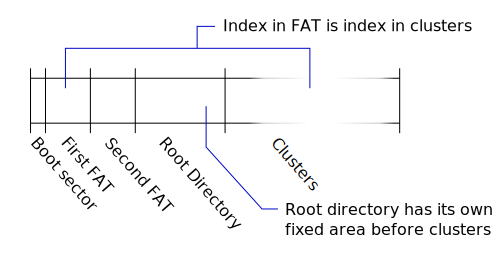
\includegraphics[width=.7\textwidth]{fat16_layout.pdf}
\caption{FAT16 Layout}
\label{fig:fat16_layout}
\end{figure}

\begin{figure}[htb]
\centering
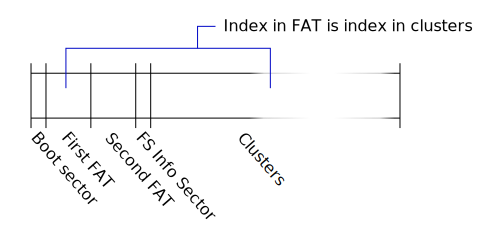
\includegraphics[width=.7\textwidth]{fat32_layout.pdf}
\caption{FAT32 Layout}
\label{fig:fat32_layout}
\end{figure}

FAT16 (and FAT12) have the particularity that the root directory is not like
other directories, but is instead inside its own area preceding the start of
the ``clusters'' area. This also implies that the maximum number of entries in
the root directory is fixed when formatting. FAT32 removes this limitation, and
adds an additional \ac{fsis} containing dynamic information about the state of
the filesystem, e.g. the amount of allocated/free space.

\section{Implementation and Limitations}

We have implemented read-only support for FAT16 and FAT32. However, because the
example \lstinline+ata_rw28+ interface only has the 28-bit {\tt READ DMA} and
{\tt WRITE DMA} commands, we can only access the first 128GB of a disk (with
512-byte sectors).

\subsection{Unicode}

While FAT 8.3 filenames are 8-bit strings, FAT long filenames use UTF-16.
Barrelfish does not have any concept of Unicode, so our FAT implementation
replaces non-\acs{ascii} characters with a question mark in directory listings,
and does not support opening files with non-\acs{ascii} filenames.

\subsection{BSD conv Functions}

To generate 8.3 filenames in the first place, we have adapted various
conversion functions from OpenBSD's msdosfs. However, our current
implementation still compares filenames case-sensitively.

\section{Caching Layer}

\begin{figure}[htb]
\centering
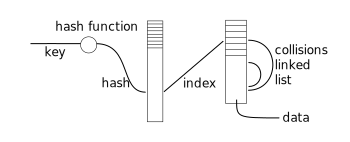
\includegraphics[width=.7\textwidth]{cache_design.pdf}
\caption{Cache Design}
\label{fig:cache_design}
\end{figure}

The FAT code uses a cache layer as a global block and cluster store,
simplifying the code and improving performance. The cache is implemented as a
fixed-size hashmap from keys to indices into a backing array. The backing array
uses doubly linked lists to handle collisions, the free list, and a list of
unused cache entries that can be freed if space is required. Clients must
acquire a reference to a cache entry, either using \lstinline+fs_cache_acquire+
if the entry is already present, or \lstinline+fs_cache_put+ when creating a
new entry. When the entry is no longer used, the client must call
\lstinline+fs_cache_release+. If the reference count for an entry sinks to
zero, it is appended to the aforementioned list of unused entries, which can be
seen as an \acs{lru} queue. Thus when \lstinline+fs_cache_put+ is called and
the cache is at its maximum capacity, it can pop the front entry from the
unused list, free its data, and use the entry for the new cache item.

The caching API consists of the following methods:
\begin{itemize}
	\item \lstinline+fs_cache_init+ and \lstinline+fs_cache_free+, for cache
		setup and teardown. The initialization method takes the maximum capacity
		of the backing array and the hashmap size. Both values must be powers of
		two.
	\item \lstinline+fs_cache_acquire+, for getting a reference to an existing
		entry.
	\item \lstinline+fs_cache_put+, for adding an item to the cache. This also
		increments the reference count as if \lstinline+fs_cache_acquire+ had
		been called.
	\item \lstinline+fs_cache_release+, for releasing a reference to an entry.
\end{itemize}

\section{VFS Interaction}

The mount URI for FAT has the format
\verb@fat<version>://<port>[+<startblock>]@, e.g. \verb@fat32://0+63@, where
{\tt version} is is either 16 or 32, {\tt port} is the \acs{ahci} port of the
device, and the optional {\tt startblock} specifies the offset the first sector
of the filesystem (the boot sector).

Unlike Barrelfish's ramfs, our FAT implementation does not share state between
multiple mounts using \acs{idc}, so with the current \acs{vfs} implementation
mounting a FAT filesystem gives the mounting domain exclusive access to the
filesystem and the whole disk. An alternative that would avoid code duplication
would be for the \acs{vfs} to allow part of its directory structure to be
exported as a service, creating a Barrelfish-internal system conceptually
similar to NFS.
